\section{Methodology \& Results}
\label{sec:method}

\subsection{Model and Distance Calculation}

To predict retinotopic maps, we constructed graph neural networks (GNNs) based on BSpline convolutions,
following the architecture of Ribeiro et. al.\ \cite{ribeiro2021}.
In this type of convolution, the piecewise polynomial functions of a BSpline update the values of the vertices
through kernel values that act as the convolutional weights.
The information entering these kernels comes from the edges between vertices.
Each edge feeds into the BSpline functions, which return the convolution weight for a given neighbor.
This weight is formed as a sum of spline parameters, each scaled by a function of the edge values,
so that the edge information itself decides how strongly a parameter contributes to the final result.

The number of parameters that contribute per input dimension is set by the kernel size, for which we chose a value of 5,
and it is these control weights that are learned during training.
How their contributions are distributed depends on the degree of the BSpline,
ranging from a linear to a smoother higher-order profile.
We used a degree of 1, meaning a control weight's influence is interpolated linearly over the interval between its neighboring knots.
Introduced by \cite{fey2018splinecnn}, this BSpline convolution lets information propagate through a graph
even when nodes differ in their number of neighbors, while still accounting for the importance of each individual neighbor.

While \cite{ribeiro2021} used the relative positions of neighbouring vertices as their edge values, we instead used the distance between two neighbouring vertices.
To investigate whether the curvature in the response distribution, which arises from cortical
magnification, can be better explained by a locally curved geometry, we changed the way this distance is calculated.
This in turn changes the input to the BSpline kernels and, with it, how information is convolved across the network.

We compared three different distance functions. The first is the commonly used Cartesian distance based on the L2 norm:
\begin{equation}
    d_{euc} = \lVert \mathrm{coord}(v_i) - \mathrm{coord}(v_j) \rVert
\end{equation}
Second, we derived a spherical distance from the great-circle arc formula, since on a sphere the shortest path between
two points always lies on a circle of radius $r$ around the origin. The curvature used to transform the Euclidean
distance is given by the parameter $k$:
\begin{equation}
    d_{sph} \approx \frac{2}{\sqrt{k}} \, \arcsin\!\left( \frac{\sqrt{k}}{2}\, d_{euc} \right)
\end{equation}
As a third option we used a hyperbolic distance derived from the distance function on a hyperboloid \cite{XXX}:
\begin{equation}
    d_{hyp} \approx \frac{2}{\sqrt{k}} \, \ln\!\left( \sqrt{k}\, d_{euc} \right)
\end{equation}
It is important to point out that both the spherical and the hyperbolic distance functions are only approximations of
the true ones, since we obtain them by transforming the Euclidean distance, stretching or compressing it as distances grow.

\subsection{Training}
We trained the graph neural network shown in Table~\ref{tab:architecture}, which stacks BSpline convolution
layers, each followed by batch normalization. Every layer except the last also applied dropout with a rate of
$10\%$. The final layer, without batch normalization, returned two values per node, which we interpreted as the
eccentricity and polar angle of that node. These predictions were compared against the ground-truth values
mapped earlier using the smooth L1 loss, which is less sensitive to outliers than a plain squared error.

The dataset of 164 meshes was split into training, validation and test sets containing $60\%$, $20\%$ and
$20\%$ of the meshes (98, 33 and 33 meshes), using the same split for all six models. We trained with a
batch size of 1 for a maximum of 100 epochs, applying early stopping with a patience of 5 epochs on the
validation loss. We used the Adam optimizer with a learning rate of $0.01$.

\begin{table}[t]
  \centering
  \caption{Architecture of the graph neural network. All convolutions are BSpline convolutions
  (\texttt{SplineConv}) with kernel size $k=5$ and pseudo-coordinate dimension $d$. Every hidden
  block applies ELU activation, batch normalisation and dropout ($p=0.1$); the final layer outputs
  the two predicted retinotopic values without activation.}
  \label{tab:architecture}
  \begin{tabular}{@{}llccccc@{}}
    \toprule
    \# & Layer & In ch. & Out ch. & Activation & BatchNorm & Dropout \\
    \midrule
    1 & SplineConv & $n_\text{res}$ & 8  & ELU & \checkmark & 0.1 \\
    2 & SplineConv & 8  & 16 & ELU & \checkmark & 0.1 \\
    3 & SplineConv & 16 & 32 & ELU & \checkmark & 0.1 \\
    4 & SplineConv & 32 & 32 & ELU & \checkmark & 0.1 \\
    5 & SplineConv & 32 & 32 & ELU & \checkmark & 0.1 \\
    6 & SplineConv & 32 & 16 & ELU & \checkmark & 0.1 \\
    7 & SplineConv & 16 & 8  & ELU & \checkmark & 0.1 \\
    8 & SplineConv & 8  & 2  & --  & --         & --  \\
    \bottomrule
  \end{tabular}
\end{table}

In total we trained six networks that differ only in the distance function used to compute the edge values
between neighboring vertices. We trained one Euclidean model, three hyperbolic models with curvatures $k$ ranging from
$0.01$ to $1.0$, and two spherical models with $k = 0.01$ and $k = 0.05$. The spherical curvature is bounded
from above by the longest edge in the graph. Since the argument of the arcsine, $\tfrac{\sqrt{k}}{2}\, d_{euc}$,
must stay within $[-1, 1]$, the curvature is constrained by $k \leq 4 / d_{max}^2$, where $d_{max}$ is the
longest edge. For larger curvatures the longest edge pushes this argument out of the valid range, which is why
only two spherical curvature values were feasible.

\subsection{Results and Discussion}

Table~\ref{tab:results} reports the test error and the number of training epochs until early stopping for each
model. The spherical model with curvature $k = 0.05$ reached the lowest test error and therefore produced the
best retinotopic map predictions. Overall, the errors were similar across models of different curvatures, and
every curved model performed at least as well as the Euclidean baseline. Training was fast for all models,
converging within a small number of epochs.

Figures~\ref{fig:predictions} and~\ref{fig:abs_error} show the predicted maps and the corresponding absolute
errors for the Euclidean model together with the best performing hyperbolic and spherical models. Comparing the
two predicted quantities, the eccentricity is recovered well by all three models, whereas the polar angle shows
clearly larger errors. These errors are especially pronounced along the line where the polar angle flips from
$360^\circ$ back to $1^\circ$. Since this jump is a discontinuity introduced by the way the data is created, it
is more likely an artefact of the data generation than a genuine zone of poor prediction.

\begin{table}[t]
  \centering
  \caption{Test error (smooth L1 loss) and number of training epochs until early stopping for each model,
  grouped by the distance function used for the edge attributes. The best result is shown in bold.}
  \label{tab:results}
  \begin{tabular}{@{}lccc@{}}
    \toprule
    Model & Curvature $k$ & Test error & Epochs \\
    \midrule
    Euclidean  & --   & 0.2291 & 8  \\
    Spherical  & 0.01 & 0.2257 & 12 \\
    Spherical  & 0.05 & \textbf{0.2045} & 21 \\
    Hyperbolic & 0.01 & 0.2082 & 15 \\
    Hyperbolic & 0.1  & 0.2101 & 16 \\
    Hyperbolic & 1.0  & 0.2080 & 18 \\
    \bottomrule
  \end{tabular}
\end{table}


\begin{figure}[t]
  \centering
  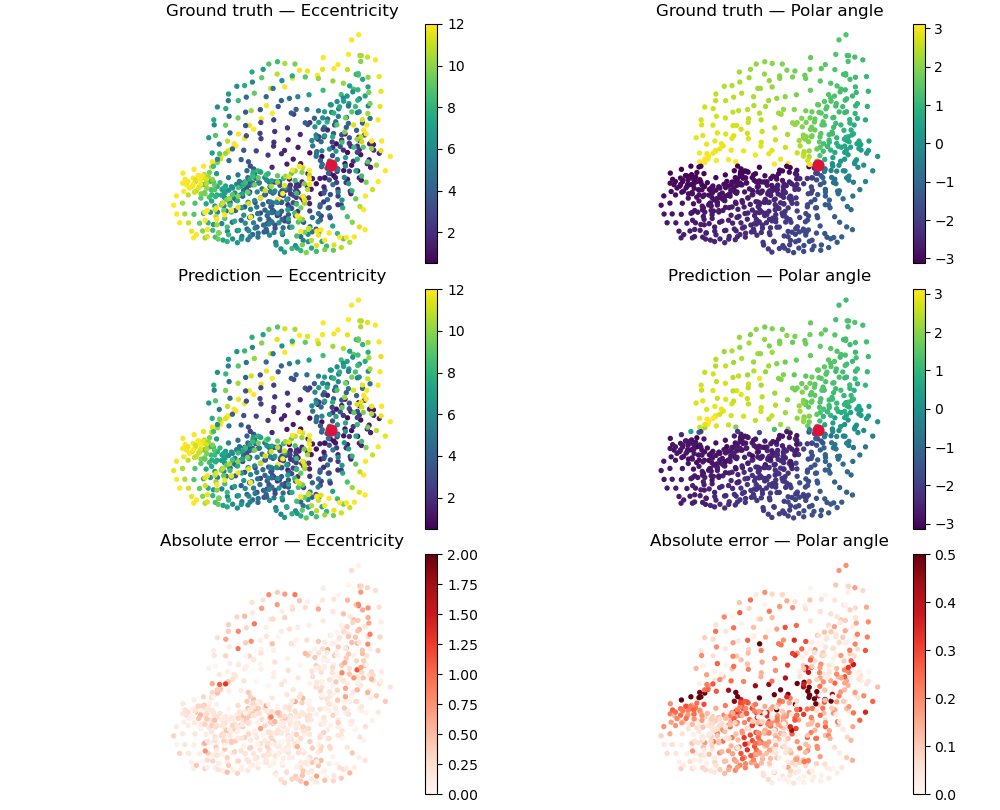
\includegraphics[width=\linewidth]{visualizations/sph_0p05.png}
  \caption{Predicted eccentricity and polar angle maps for the Euclidean model and the best performing
  hyperbolic and spherical models. The eccentricity is recovered well by all three models, while larger
  deviations appear in the polar angle.}
  \label{fig:predictions}
\end{figure}

\begin{figure}[t]
  \centering
  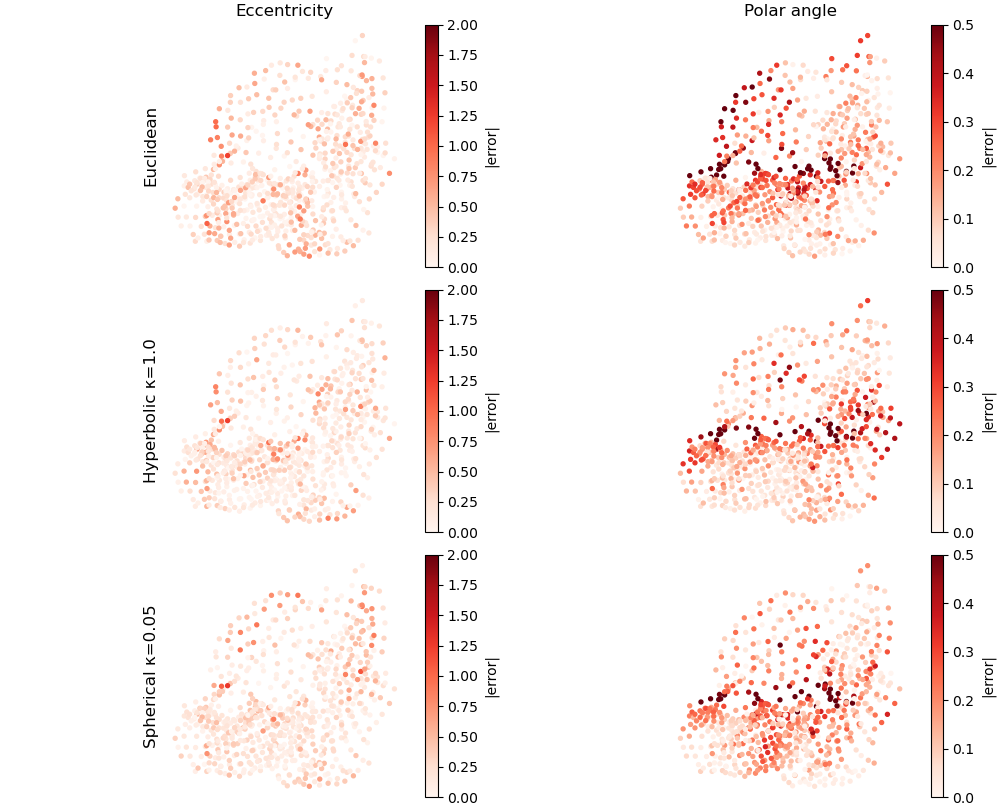
\includegraphics[width=\linewidth]{visualizations/absolut_error.png}
  \caption{Absolute prediction error for the Euclidean model and the best performing hyperbolic and spherical
  models. Warmer colors indicate larger errors.}
  \label{fig:abs_error}
\end{figure}

Including curvature in the edge distances improved the recovery of the retinotopic map compared to the Euclidean
baseline. Nevertheless, a clear and consistent effect of curvature could not be identified, since the differences
between the curved models were small and did not follow an obvious trend with the curvature value. These results
should also be read in light of the limitations of our setup. Unfortunately, we were not able to make an
extensive hyperparameter selection due to our limited computing resources, and for the same reason the size of
the model was kept small.

Two directions stand out for future work. First, the direction of an edge could be added as a further edge
attribute, so that the kernel receives not only the distance but also the orientation between neighboring nodes.
Second, embedding layers could be added to the network to map nodes onto the model manifold directly, rather than
only encoding the geometry through the edge distances.